\documentclass[10pt]{article}
\usepackage[polish]{babel}
\usepackage[utf8]{inputenc}
\usepackage[T1]{fontenc}
\usepackage{graphicx}
\usepackage[export]{adjustbox}
\graphicspath{ {./images/} }
\usepackage{amsmath}
\usepackage{amsfonts}
\usepackage{amssymb}
\usepackage[version=4]{mhchem}
\usepackage{stmaryrd}
\usepackage{multirow}

\title{EGZAMIN MATURALNY Z MATEMATYKI POZIOM PODSTAWOWY }

\author{}
\date{}


\newcommand\Varangle{\mathop{{<\!\!\!\!\!\text{\small)}}\:}\nolimits}

\begin{document}
\maketitle
\begin{center}
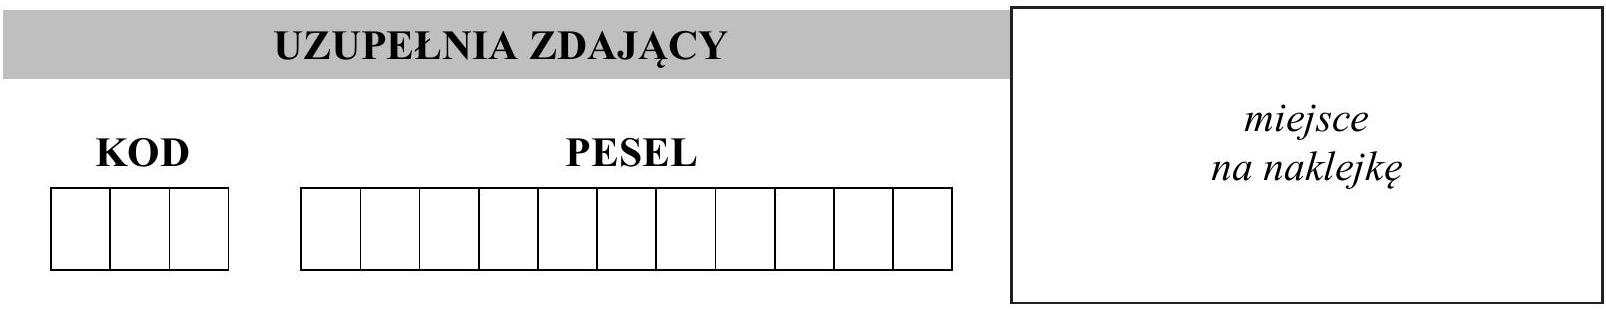
\includegraphics[max width=\textwidth]{2024_11_21_7b5527312ea89ae66fd0g-01(1)}
\end{center}

\section*{Data: 5 maja 2017 r.}
Godzina rozpoczeclia: 9:00\\
CZAS PRACY: \(\mathbf{1 7 0}\) minut\\
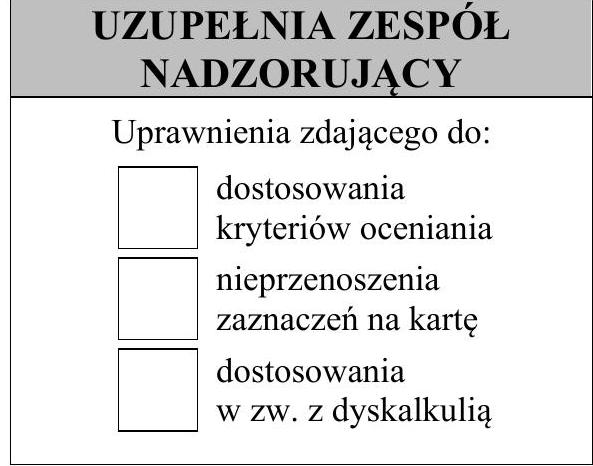
\includegraphics[max width=\textwidth, center]{2024_11_21_7b5527312ea89ae66fd0g-01}

LICZba PunKTÓW dO UZYSKANIA: 50

\section*{Instrukcja dla zdającego}
\begin{enumerate}
  \item Sprawdź, czy arkusz egzaminacyjny zawiera 26 stron (zadania 1-34).
\end{enumerate}

Ewentualny brak zgłoś przewodniczącemu zespołu nadzorującego egzamin.\\
2. Rozwiązania zadań i odpowiedzi wpisuj w miejscu na to przeznaczonym.\\
3. Odpowiedzi do zadań zamkniętych (1-25) zaznacz na karcie odpowiedzi, w części karty przeznaczonej dla zdającego. Zamaluj \(\square\) pola do tego\\

\includegraphics[max width=\textwidth, center]{2024_11_21_7b5527312ea89ae66fd0g-01(2)}\\
4. Pamiętaj, że pominięcie argumentacji lub istotnych obliczeń w rozwiązaniu zadania otwartego (26-34) może spowodować, że za to rozwiązanie nie otrzymasz pełnej liczby punktów.\\
5. Pisz czytelnie i używaj tylko długopisu lub pióra z czarnym tuszem lub atramentem.\\
6. Nie używaj korektora, a błędne zapisy wyraźnie przekreśl.\\
7. Pamiętaj, że zapisy w brudnopisie nie będą oceniane.\\
8. Możesz korzystać z zestawu wzorów matematycznych, cyrkla i linijki, a także z kalkulatora prostego.\\
9. Na tej stronie oraz na karcie odpowiedzi wpisz swój numer PESEL i przyklej naklejkę z kodem.\\
10. Nie wpisuj żadnych znaków w części przeznaczonej dla egzaminatora.\\

\includegraphics[max width=\textwidth, center]{2024_11_21_7b5527312ea89ae66fd0g-01(3)}

W zadaniach od 1. do 25. wybierz i zaznacz na karcie odpowiedzi poprawna odpowiedź.

\section*{Zadanie 1. (0-1)}
Liczba \(5^{8} \cdot 16^{-2}\) jest równa\\
A. \(\left(\frac{5}{2}\right)^{8}\)\\
B. \(\frac{5}{2}\)\\
C. \(10^{8}\)\\
D. 10

\section*{Zadanie 2. (0-1)}
Liczba \(\sqrt[3]{54}-\sqrt[3]{2}\) jest równa\\
A. \(\sqrt[3]{52}\)\\
B. 3\\
C. \(2 \sqrt[3]{2}\)\\
D. 2

\section*{Zadanie 3. (0-1)}
Liczba \(2 \log _{2} 3-2 \log _{2} 5\) jest równa\\
A. \(\log _{2} \frac{9}{25}\)\\
B. \(\log _{2} \frac{3}{5}\)\\
C. \(\log _{2} \frac{9}{5}\)\\
D. \(\log _{2} \frac{6}{25}\)

\section*{Zadanie 4. (0-1)}
Liczba osobników pewnego zagrożonego wyginięciem gatunku zwierząt wzrosła w stosunku do liczby tych zwierząt z 31 grudnia 2011 r. o \(120 \%\) i obecnie jest równa 8910 . Ile zwierząt liczyła populacja tego gatunku w ostatnim dniu 2011 roku?\\
A. 4050\\
B. 1782\\
C. 7425\\
D. 7128

\section*{Zadanie 5. (0-1)}
Równość \((x \sqrt{2}-2)^{2}=(2+\sqrt{2})^{2}\) jest\\
A. prawdziwa dla \(x=-\sqrt{2}\).\\
B. prawdziwa dla \(x=\sqrt{2}\).\\
C. prawdziwa dla \(x=-1\).\\
D. fałszywa dla każdej liczby \(x\).

BRUDNOPIS (nie podlega ocenie)\\

\includegraphics[max width=\textwidth, center]{2024_11_21_7b5527312ea89ae66fd0g-03}

\section*{Zadanie 6. (0-1)}
Do zbioru rozwiązań nierówności \(\left(x^{4}+1\right)(2-x)>0\) nie należy liczba\\
A. -3\\
B. -1\\
C. 1\\
D. 3

\section*{Zadanie 7. (0-1)}
Wskaż rysunek, na którym jest przedstawiony zbiór wszystkich rozwiązań nierówności \(2-3 x \geq 4\).\\
A.\\
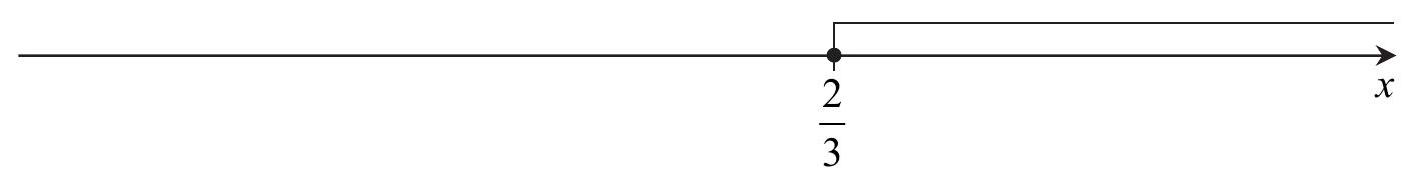
\includegraphics[max width=\textwidth, center]{2024_11_21_7b5527312ea89ae66fd0g-04(2)}\\
B.\\
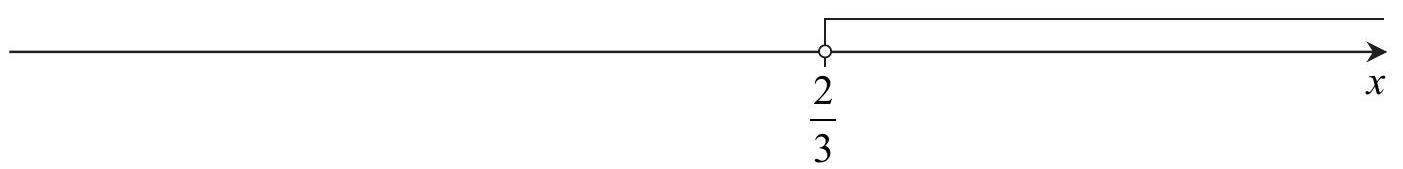
\includegraphics[max width=\textwidth, center]{2024_11_21_7b5527312ea89ae66fd0g-04(1)}\\
C.\\
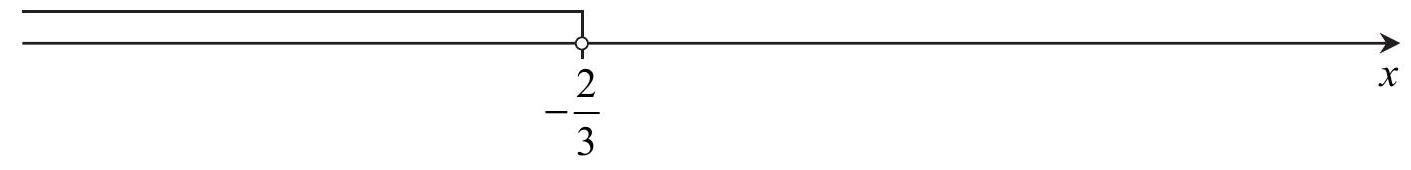
\includegraphics[max width=\textwidth, center]{2024_11_21_7b5527312ea89ae66fd0g-04}\\
D.\\
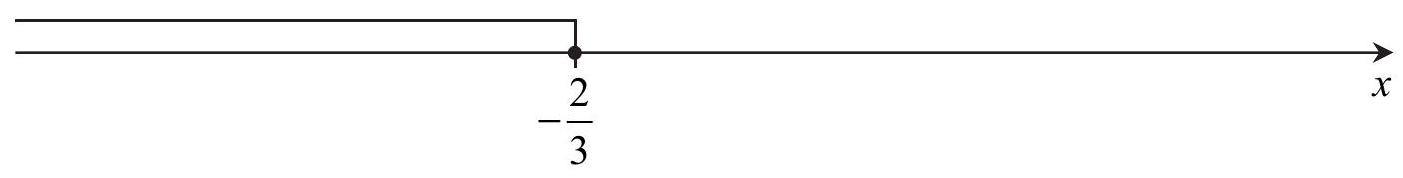
\includegraphics[max width=\textwidth, center]{2024_11_21_7b5527312ea89ae66fd0g-04(3)}

\section*{Zadanie 8. (0-1)}
Równanie \(x\left(x^{2}-4\right)\left(x^{2}+4\right)=0\) z niewiadomą \(x\)\\
A. nie ma rozwiązań w zbiorze liczb rzeczywistych.\\
B. ma dokładnie dwa rozwiązania w zbiorze liczb rzeczywistych.\\
C. ma dokładnie trzy rozwiązania w zbiorze liczb rzeczywistych.\\
D. ma dokładnie pięć rozwiązań w zbiorze liczb rzeczywistych.

\section*{Zadanie 9. (0-1)}
Miejscem zerowym funkcji liniowej \(f(x)=\sqrt{3}(x+1)-12\) jest liczba\\
A. \(\sqrt{3}-4\)\\
B. \(-2 \sqrt{3}+1\)\\
C. \(4 \sqrt{3}-1\)\\
D. \(-\sqrt{3}+12\)

\section*{BRUDNOPIS (nie podlega ocenie)}
\begin{center}

\includegraphics[max width=\textwidth]{2024_11_21_7b5527312ea89ae66fd0g-05}
\end{center}

\section*{Zadanie 10. (0-1)}
Na rysunku przedstawiono fragment wykresu funkcji kwadratowej \(f(x)=a x^{2}+b x+c\), której miejsca zerowe to: -3 i 1.\\
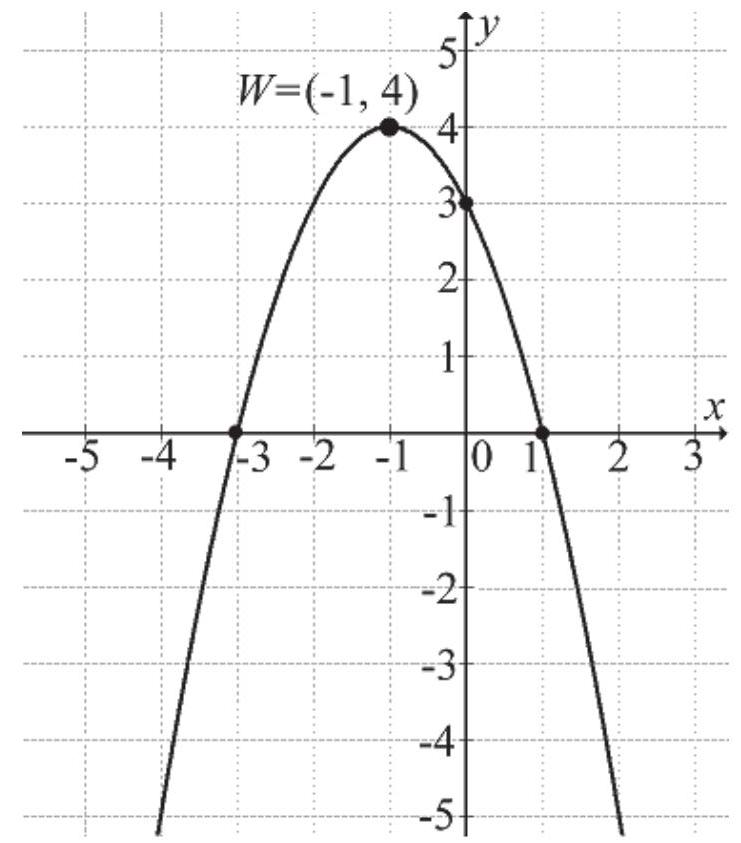
\includegraphics[max width=\textwidth, center]{2024_11_21_7b5527312ea89ae66fd0g-06}

Współczynnik \(c\) we wzorze funkcji \(f\) jest równy\\
A. 1\\
B. 2\\
C. 3\\
D. 4

\section*{Zadanie 11. (0-1)}
Na rysunku przedstawiono fragment wykresu funkcji wykładniczej \(f\) określonej wzorem \(f(x)=a^{x}\). Punkt \(A=(1,2)\) należy do tego wykresu funkcji.\\
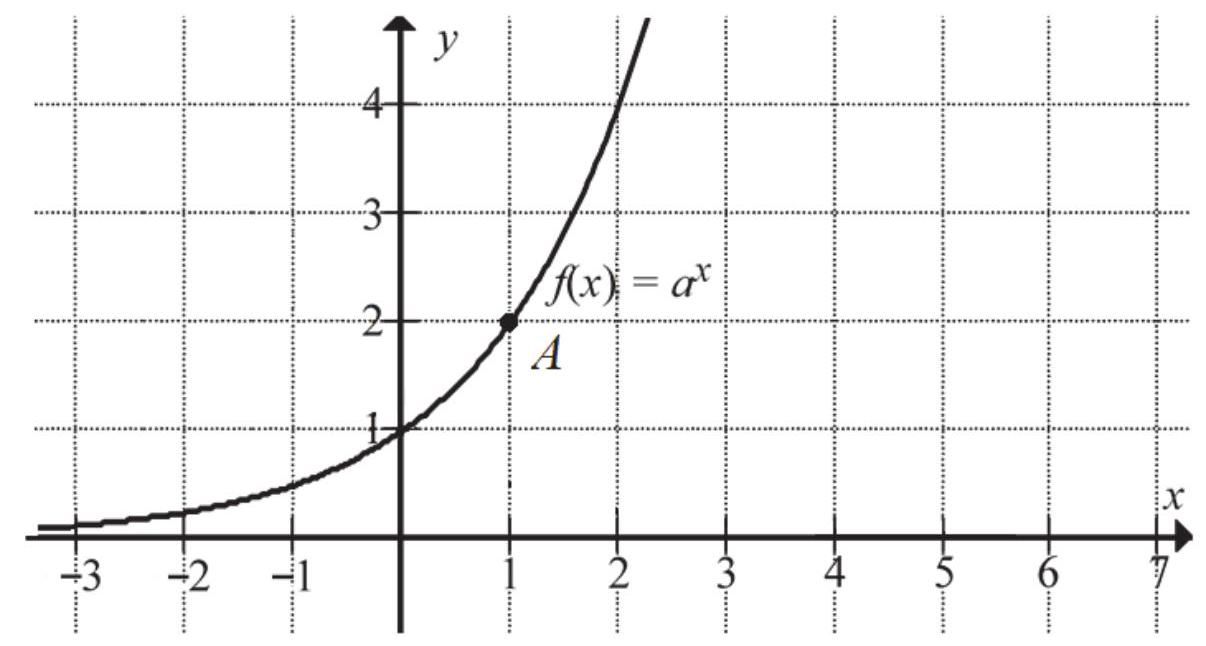
\includegraphics[max width=\textwidth, center]{2024_11_21_7b5527312ea89ae66fd0g-06(1)}

Podstawa a potęgi jest równa\\
A. \(-\frac{1}{2}\)\\
B. \(\frac{1}{2}\)\\
C. -2\\
D. 2

BRUDNOPIS (nie podlega ocenie)\\

\includegraphics[max width=\textwidth, center]{2024_11_21_7b5527312ea89ae66fd0g-07}

\section*{Zadanie 12. (0-1)}
W ciągu arytmetycznym \(\left(a_{n}\right)\), określonym dla \(n \geq 1\), dane są: \(a_{1}=5, a_{2}=11\). Wtedy\\
A. \(a_{14}=71\)\\
B. \(a_{12}=71\)\\
C. \(a_{11}=71\)\\
D. \(a_{10}=71\)

\section*{Zadanie 13. (0-1)}
Dany jest trzywyrazowy ciąg geometryczny (24, 6, a-1). Stąd wynika, że\\
A. \(a=\frac{5}{2}\)\\
B. \(a=\frac{2}{5}\)\\
C. \(a=\frac{3}{2}\)\\
D. \(a=\frac{2}{3}\)

\section*{Zadanie 14. (0-1)}
Jeśli \(m=\sin 50^{\circ}\), to\\
A. \(m=\sin 40^{\circ}\)\\
B. \(m=\cos 40^{\circ}\)\\
C. \(m=\cos 50^{\circ}\)\\
D. \(m=\operatorname{tg} 50^{\circ}\)

\section*{Zadanie 15. (0-1)}
Na okręgu o środku w punkcie \(O\) leży punkt \(C\) (zobacz rysunek). Odcinek \(A B\) jest średnicą tego okręgu. Zaznaczony na rysunku kąt środkowy \(\alpha\) ma miarę\\
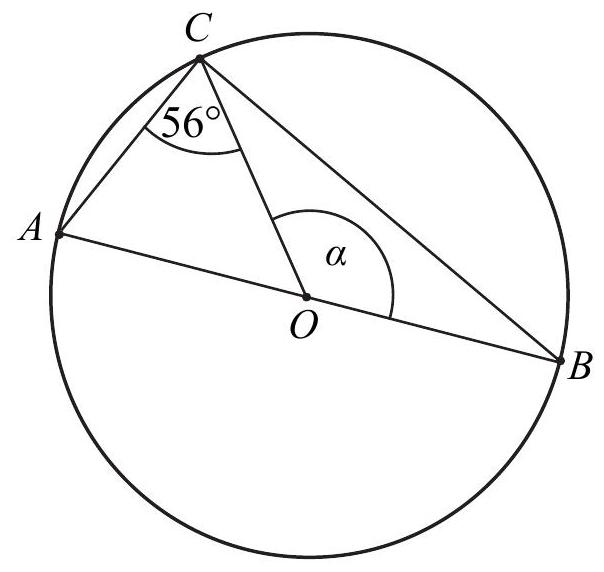
\includegraphics[max width=\textwidth, center]{2024_11_21_7b5527312ea89ae66fd0g-08}\\
A. \(116^{\circ}\)\\
B. \(114^{\circ}\)\\
C. \(112^{\circ}\)\\
D. \(110^{\circ}\)

BRUDNOPIS (nie podlega ocenie)\\

\includegraphics[max width=\textwidth, center]{2024_11_21_7b5527312ea89ae66fd0g-09}

\section*{Zadanie 16. (0-1)}
W trójkącie \(A B C\) punkt \(D\) leży na boku \(B C\), a punkt \(E\) leży na boku \(A B\). Odcinek \(D E\) jest równoległy do boku \(A C\), a ponadto \(|B D|=10,|B C|=12\) i \(|A C|=24\) (zobacz rysunek).\\
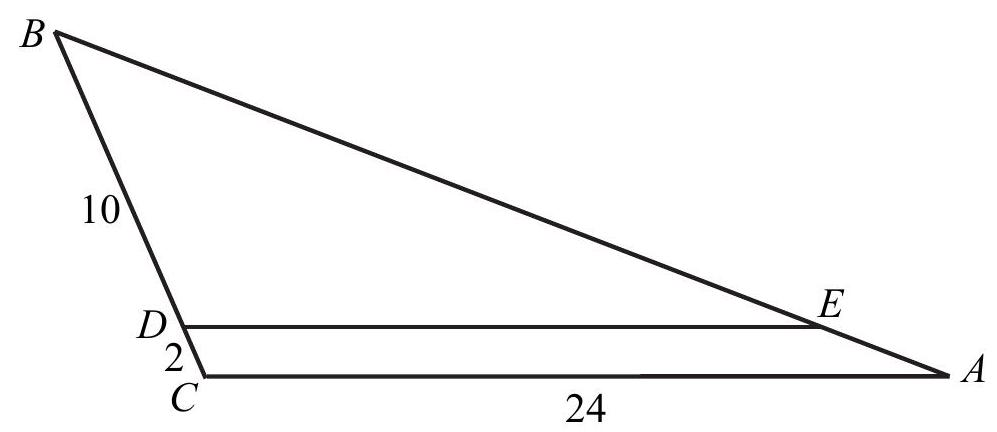
\includegraphics[max width=\textwidth, center]{2024_11_21_7b5527312ea89ae66fd0g-10}

Długość odcinka \(D E\) jest równa\\
A. 22\\
B. 20\\
C. 12\\
D. 11

\section*{Zadanie 17. (0-1)}
Obwód trójkąta \(A B C\), przedstawionego na rysunku, jest równy\\
A. \(\left(3+\frac{\sqrt{3}}{2}\right) a\)\\
B. \(\left(2+\frac{\sqrt{2}}{2}\right) a\)\\
C. \((3+\sqrt{3}) a\)\\
D. \((2+\sqrt{2}) a\)

BRUDNOPIS (nie podlega ocenie)\\

\includegraphics[max width=\textwidth, center]{2024_11_21_7b5527312ea89ae66fd0g-11}

\section*{Zadanie 18. (0-1)}
Na rysunku przedstawiona jest prosta \(k\), przechodząca przez punkt \(A=(2,-3)\) i przez początek układu współzzędnych, oraz zaznaczony jest kąt \(\alpha\) nachylenia tej prostej do osi \(O x\).\\
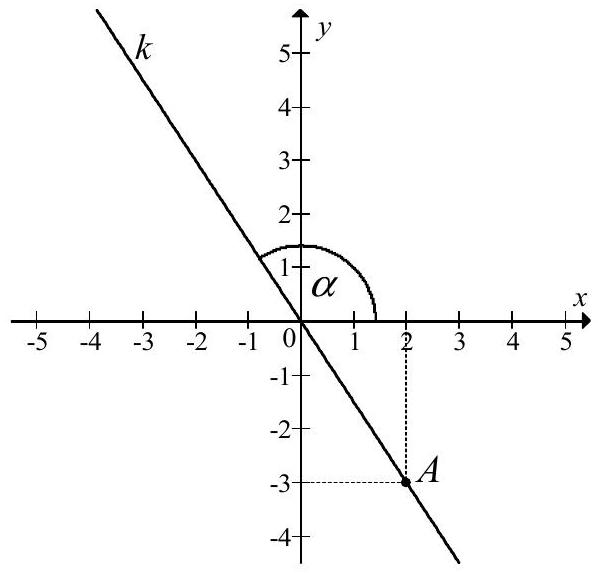
\includegraphics[max width=\textwidth, center]{2024_11_21_7b5527312ea89ae66fd0g-12}

Zatem\\
A. \(\operatorname{tg} \alpha=-\frac{2}{3}\)\\
B. \(\operatorname{tg} \alpha=-\frac{3}{2}\)\\
C. \(\operatorname{tg} \alpha=\frac{2}{3}\)\\
D. \(\operatorname{tg} \alpha=\frac{3}{2}\)

\section*{Zadanie 19. (0-1)}
Na płaszczyźnie z układem współrzędnych proste \(k\) i \(l\) przecinają się pod kątem prostym w punkcie \(A=(-2,4)\). Prosta \(k\) jest określona równaniem \(y=-\frac{1}{4} x+\frac{7}{2}\). Zatem prostą \(l\) opisuje równanie\\
A. \(y=\frac{1}{4} x+\frac{7}{2}\)\\
B. \(y=-\frac{1}{4} x-\frac{7}{2}\)\\
C. \(y=4 x-12\)\\
D. \(y=4 x+12\)

\section*{Zadanie 20. (0-1)}
Dany jest okrąg o środku \(S=(2,3)\) i promieniu \(r=5\). Który z podanych punktów leży na tym okręgu?\\
A. \(A=(-1,7)\)\\
B. \(B=(2,-3)\)\\
C. \(C=(3,2)\)\\
D. \(\quad D=(5,3)\)

\section*{Zadanie 21. (0-1)}
Pole powierzchni całkowitej graniastosłupa prawidłowego czworokątnego, w którym wysokość jest 3 razy dłuższa od krawędzi podstawy, jest równe 140. Zatem krawędź podstawy tego graniastosłupa jest równa\\
A. \(\sqrt{10}\)\\
B. \(3 \sqrt{10}\)\\
C. \(\sqrt{42}\)\\
D. \(3 \sqrt{42}\)

BRUDNOPIS (nie podlega ocenie)\\

\includegraphics[max width=\textwidth, center]{2024_11_21_7b5527312ea89ae66fd0g-13}

Promień \(A S\) podstawy walca jest równy wysokości \(O S\) tego walca. Sinus kąta \(O A S\) (zobacz rysunek) jest równy\\
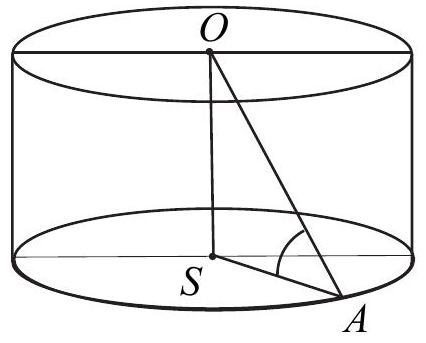
\includegraphics[max width=\textwidth, center]{2024_11_21_7b5527312ea89ae66fd0g-14}\\
A. \(\frac{\sqrt{3}}{2}\)\\
B. \(\frac{\sqrt{2}}{2}\)\\
C. \(\frac{1}{2}\)\\
D. 1

\section*{Zadanie 23. (0-1)}
Dany jest stożek o wysokości 4 i średnicy podstawy 12. Objętość tego stożka jest równa\\
A. \(576 \pi\)\\
B. \(192 \pi\)\\
C. \(144 \pi\)\\
D. \(48 \pi\)

\section*{Zadanie 24. (0-1)}
Srednia arytmetyczna ośmiu liczb: \(3,5,7,9, x, 15,17,19\) jest równa 11 . Wtedy\\
A. \(x=1\)\\
B. \(x=2\)\\
C. \(x=11\)\\
D. \(x=13\)

\section*{Zadanie 25. (0-1)}
Ze zbioru dwudziestu czterech kolejnych liczb naturalnych od 1 do 24 losujemy jedną liczbę. Niech \(A\) oznacza zdarzenie, że wylosowana liczba będzie dzielnikiem liczby 24. Wtedy prawdopodobieństwo zdarzenia \(A\) jest równe\\
A. \(\frac{1}{4}\)\\
B. \(\frac{1}{3}\)\\
C. \(\frac{1}{8}\)\\
D. \(\frac{1}{6}\)

BRUDNOPIS (nie podlega ocenie)\\

\includegraphics[max width=\textwidth, center]{2024_11_21_7b5527312ea89ae66fd0g-15}

\section*{Zadanie 26. (0-2)}
Rozwiąż nierówność \(8 x^{2}-72 x \leq 0\).

\begin{center}
\begin{tabular}{|c|c|c|c|c|c|c|c|c|c|c|c|c|c|c|c|c|c|c|c|c|c|}
\hline
 &  &  &  &  &  &  &  &  &  &  &  &  &  &  &  &  &  &  &  &  &  \\
\hline
 &  &  &  &  &  &  &  &  &  &  &  &  &  &  &  &  &  &  &  &  &  \\
\hline
 &  &  &  &  &  &  &  &  &  &  &  &  &  &  &  &  &  &  &  &  &  \\
\hline
 &  &  &  &  &  &  &  &  &  &  &  &  &  &  &  &  &  &  &  &  &  \\
\hline
 &  &  &  &  &  &  &  &  &  &  &  &  &  &  &  &  &  &  &  &  &  \\
\hline
 &  &  &  &  &  &  &  &  &  &  &  &  &  &  &  &  &  &  &  &  &  \\
\hline
 &  &  &  &  &  &  &  &  &  &  &  &  &  &  &  &  &  &  &  &  &  \\
\hline
 &  &  &  &  &  &  &  &  &  &  &  &  &  &  &  &  &  &  &  &  &  \\
\hline
 &  &  &  &  &  &  &  &  &  &  &  &  &  &  &  &  &  &  &  &  &  \\
\hline
 &  &  &  &  &  &  &  &  &  &  &  &  &  &  &  &  &  &  &  &  &  \\
\hline
 &  &  &  &  &  &  &  &  &  &  &  &  &  &  &  &  &  &  &  &  &  \\
\hline
 &  &  &  &  &  &  &  &  &  &  &  &  &  &  &  &  &  &  &  &  &  \\
\hline
 &  &  &  &  &  &  &  &  &  &  &  &  &  &  &  &  &  &  &  &  &  \\
\hline
 &  &  &  &  &  &  &  &  &  &  &  &  &  &  &  &  &  &  &  &  &  \\
\hline
 &  &  &  &  &  &  &  &  &  &  &  &  &  &  &  &  &  &  &  &  &  \\
\hline
 &  &  &  &  &  &  &  &  &  &  &  &  &  &  &  &  &  &  &  &  &  \\
\hline
 &  &  &  &  &  &  &  &  &  &  &  &  &  &  &  &  &  &  &  &  &  \\
\hline
 &  &  &  &  &  &  &  &  &  &  &  &  &  &  &  &  &  &  &  &  &  \\
\hline
 &  &  &  &  &  &  &  &  &  &  &  &  &  &  &  &  &  &  &  &  &  \\
\hline
 &  &  &  &  &  &  &  &  &  &  &  &  &  &  &  &  &  &  &  &  &  \\
\hline
 &  &  &  &  &  &  &  &  &  &  &  &  &  &  &  &  &  &  &  &  &  \\
\hline
 &  &  &  &  &  &  &  &  &  &  &  &  &  &  &  &  &  &  &  &  &  \\
\hline
 &  &  &  &  &  &  &  &  &  &  &  &  &  &  &  &  &  &  &  &  &  \\
\hline
 &  &  &  &  &  &  &  &  &  &  &  &  &  &  &  &  &  &  &  &  &  \\
\hline
 &  &  &  &  &  &  &  &  &  &  &  &  &  &  &  &  &  &  &  &  &  \\
\hline
 &  &  &  &  &  &  &  &  &  &  &  &  &  &  &  &  &  &  &  &  &  \\
\hline
 &  &  &  &  &  &  &  &  &  &  &  &  &  &  &  &  &  &  &  &  &  \\
\hline
 &  &  &  &  &  &  &  &  &  &  &  &  &  &  &  &  &  &  &  &  &  \\
\hline
 &  &  &  &  &  &  &  &  &  &  &  &  &  &  &  &  &  &  &  &  &  \\
\hline
 &  &  &  &  &  &  &  &  &  &  &  &  &  &  &  &  &  &  &  &  &  \\
\hline
 &  &  &  &  &  &  &  &  &  &  &  &  &  &  &  &  &  &  &  &  &  \\
\hline
 &  &  &  &  &  &  &  &  &  &  &  &  &  &  &  &  &  &  &  &  &  \\
\hline
 &  &  &  &  &  &  &  &  &  &  &  &  &  &  &  &  &  &  &  &  &  \\
\hline
 &  &  &  &  &  &  &  &  &  &  &  &  &  &  &  &  &  &  &  &  &  \\
\hline
 &  &  &  &  &  &  &  &  &  &  &  &  &  &  &  &  &  &  &  &  &  \\
\hline
 &  &  &  &  &  &  &  &  &  &  &  &  &  &  &  &  &  &  &  &  &  \\
\hline
 &  &  &  &  &  &  &  &  &  &  &  &  &  &  &  &  &  &  &  &  &  \\
\hline
 &  &  &  &  &  &  &  &  &  &  &  &  &  &  &  &  &  &  &  &  &  \\
\hline
 &  &  &  &  &  &  &  &  &  &  &  &  &  &  &  &  &  &  &  &  &  \\
\hline
 &  &  &  &  &  &  &  &  &  &  &  &  &  &  &  &  &  &  &  &  &  \\
\hline
 &  &  &  &  &  &  &  &  &  &  &  &  &  &  &  &  &  &  &  &  &  \\
\hline
 &  &  &  &  &  &  &  &  &  &  &  &  &  &  &  &  &  &  &  &  &  \\
\hline
 &  &  &  &  &  &  &  &  &  &  &  &  &  &  &  &  &  &  &  &  &  \\
\hline
\end{tabular}
\end{center}

Odpowiedź:

\section*{Zadanie 27. (0-2)}
Wykaż, że liczba \(4^{2017}+4^{2018}+4^{2019}+4^{2020}\) jest podzielna przez 17 .\\
\(\qquad\)

\begin{center}
\begin{tabular}{|c|l|c|c|}
\hline
\multirow{2}{*}{\begin{tabular}{c}
Wypełnia \\
egzaminator \\
\end{tabular}} & Nr zadania & 26. & 27. \\
\cline { 2 - 4 }
 & Maks. liczba pkt & 2 & 2 \\
\cline { 2 - 4 }
 & Uzyskana liczba pkt &  &  \\
\hline
\end{tabular}
\end{center}

\section*{Zadanie 28. (0-2)}
Dane są dwa okręgi o środkach w punktach \(P\) i \(R\), styczne zewnętrznie w punkcie \(C\). Prosta \(A B\) jest styczna do obu okręgów odpowiednio w punktach \(A\) i \(B\) oraz \(|\Varangle A P C|=\alpha\) i \(|\Varangle A B C|=\beta\) (zobacz rysunek). Wykaż, że \(\alpha=180^{\circ}-2 \beta\).\\
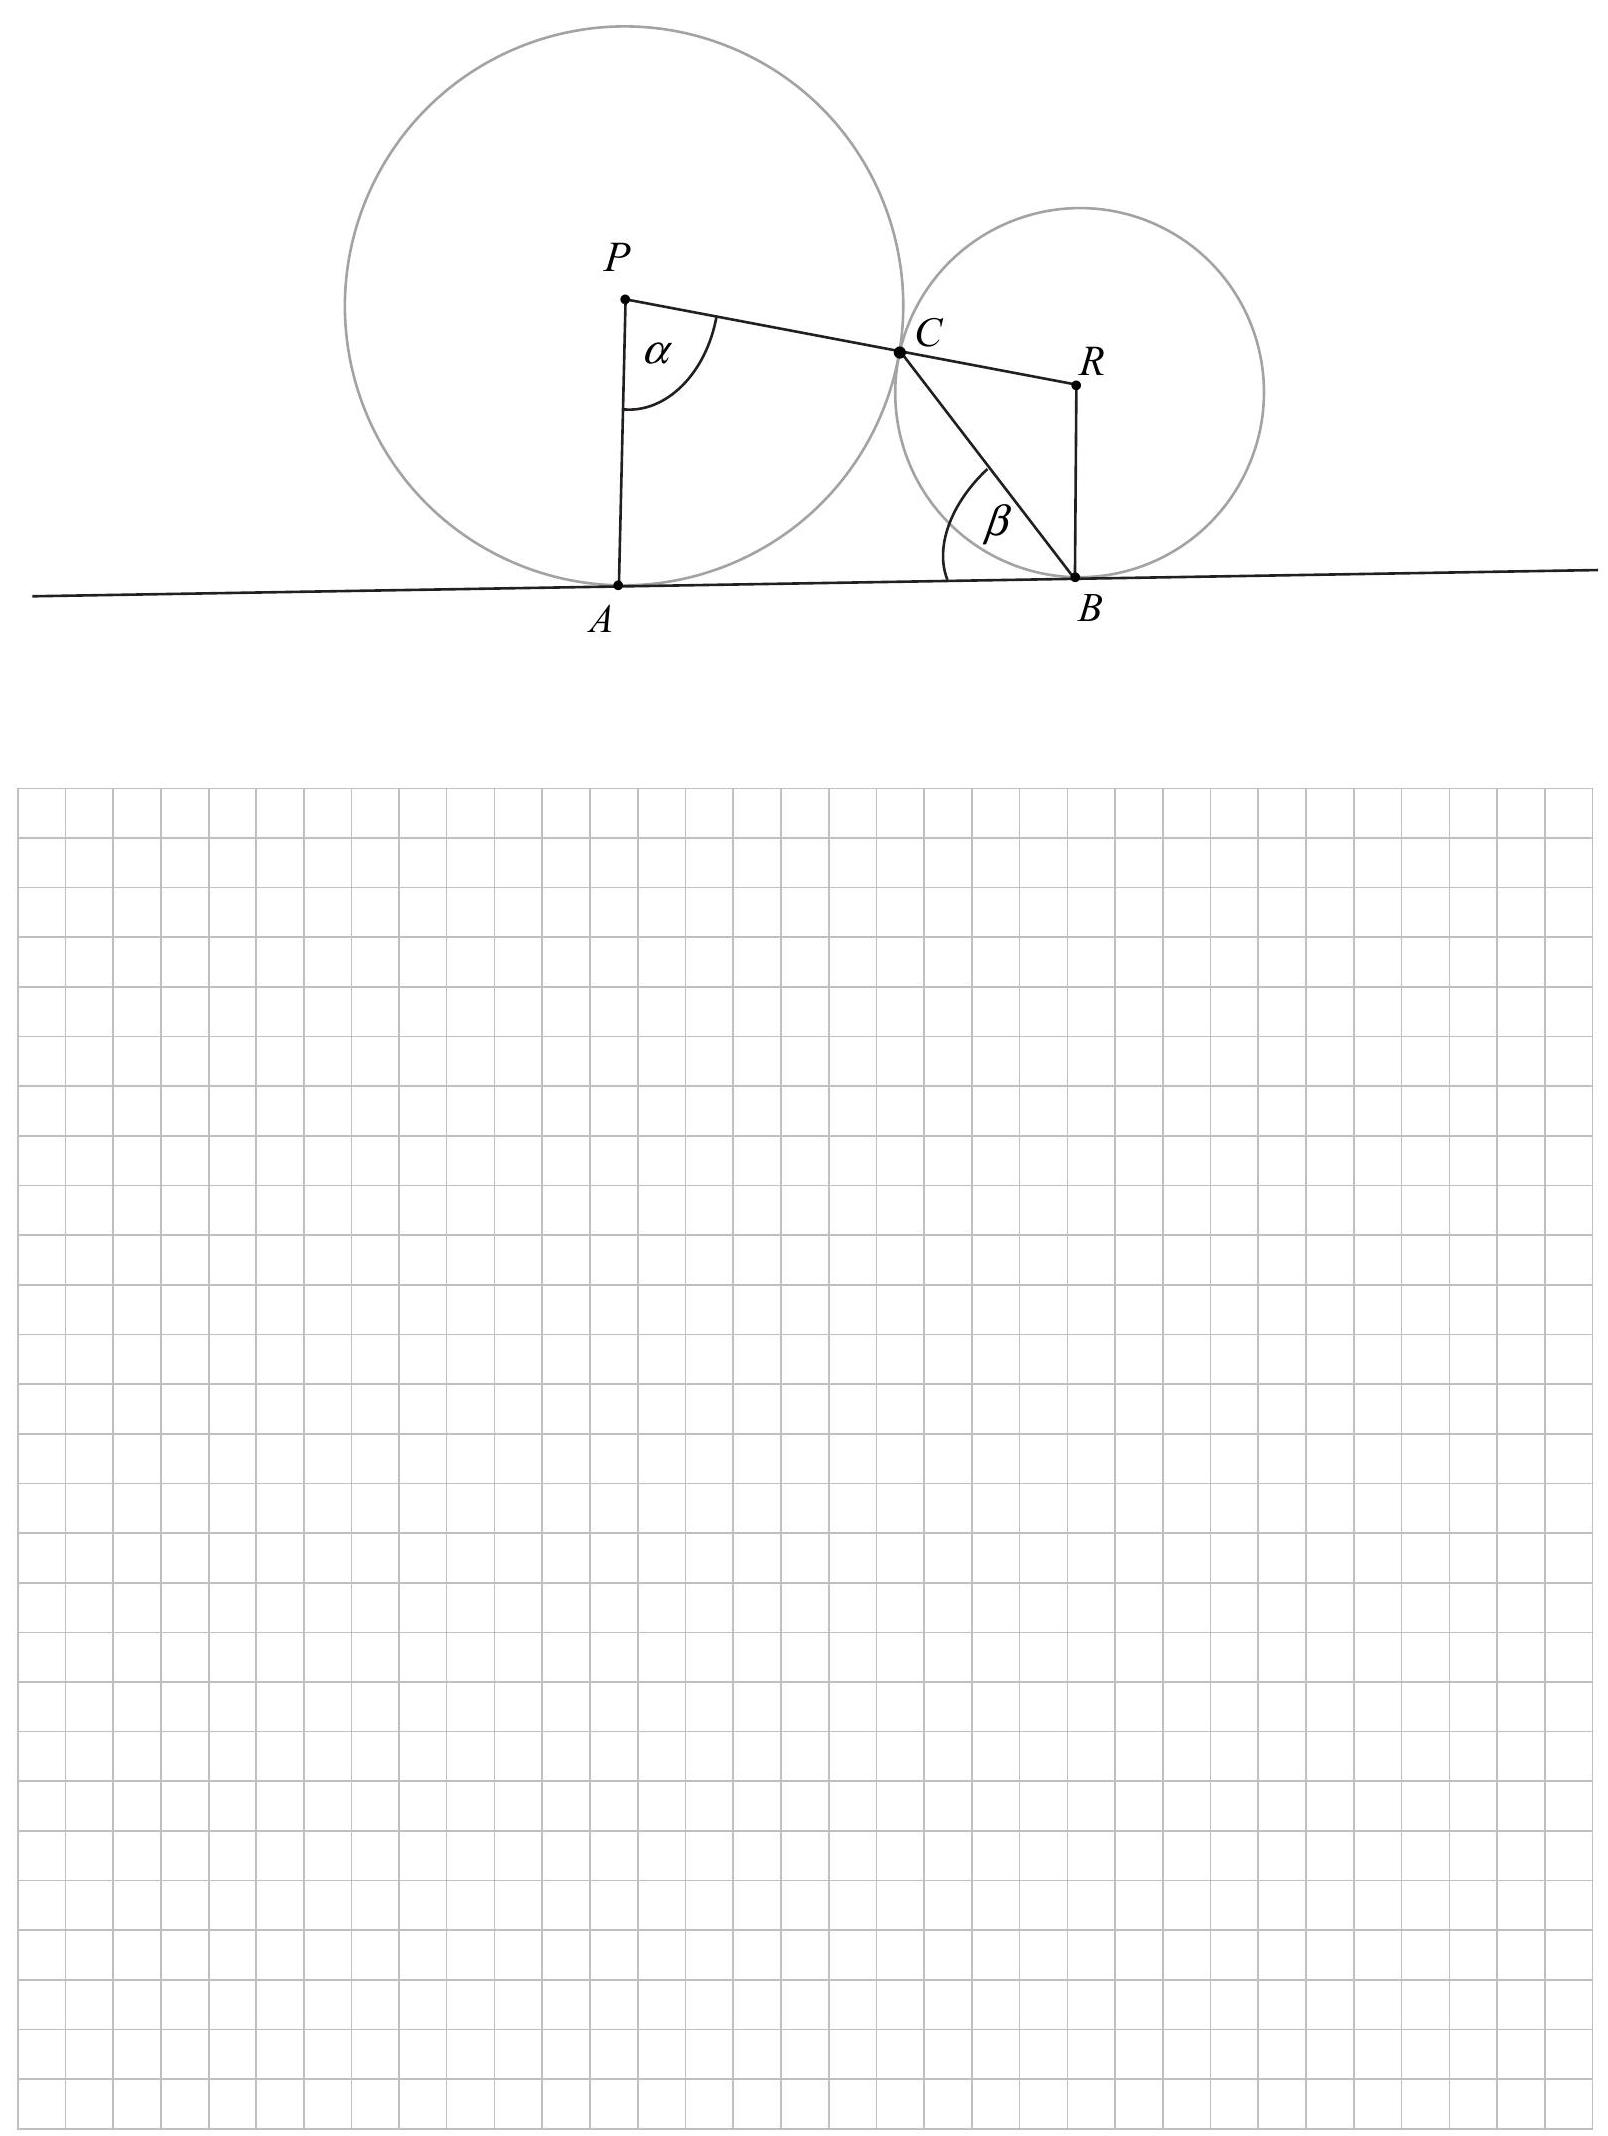
\includegraphics[max width=\textwidth, center]{2024_11_21_7b5527312ea89ae66fd0g-18}

\section*{Zadanie 29. (0-4)}
Funkcja kwadratowa \(f\) jest określona dla wszystkich liczb rzeczywistych \(x\) wzorem \(f(x)=a x^{2}+b x+c\). Największa wartość funkcji \(f\) jest równa 6 oraz \(f(-6)=f(0)=\frac{3}{2}\).\\
Oblicz wartość współczynnika \(a\).\\

\includegraphics[max width=\textwidth, center]{2024_11_21_7b5527312ea89ae66fd0g-19}

Odpowiedź:

\begin{center}
\begin{tabular}{|c|l|c|c|}
\hline
\multirow{2}{*}{\begin{tabular}{l}
Wypelnia \\
egzaminator \\
\end{tabular}} & Nr zadania & 28. & 29. \\
\cline { 2 - 4 }
 & Maks. liczba pkt & 2 & 4 \\
\cline { 2 - 4 }
 & Uzyskana liczba pkt &  &  \\
\hline
\end{tabular}
\end{center}

\section*{Zadanie 30. (0-2)}
Przeciwprostokątna trójkąta prostokątnego ma długość 26 cm , a jedna z przyprostokątnych jest o 14 cm dłuższa od drugiej. Oblicz obwód tego trójkąta.\\

\includegraphics[max width=\textwidth, center]{2024_11_21_7b5527312ea89ae66fd0g-20}

Odpowiedź: \(\qquad\)

\section*{Zadanie 31. (0-2)}
W ciągu arytmetycznym \(\left(a_{n}\right)\), określonym dla \(n \geq 1\), dane są: wyraz \(a_{1}=8\) i suma trzech początkowych wyrazów tego ciągu \(S_{3}=33\). Oblicz różnicę \(a_{16}-a_{13}\).\\

\includegraphics[max width=\textwidth, center]{2024_11_21_7b5527312ea89ae66fd0g-21}

Odpowiedź:

\begin{center}
\begin{tabular}{|c|l|c|c|}
\hline
\multirow{2}{*}{\begin{tabular}{c}
Wypetnia \\
egzaminator \\
\end{tabular}} & Nr zadania & 30. & 31. \\
\cline { 2 - 4 }
 & Maks. liczba pkt & \(\mathbf{2}\) & \(\mathbf{2}\) \\
\cline { 2 - 4 }
 & Uzyskana liczba pkt &  &  \\
\hline
\end{tabular}
\end{center}

\section*{Zadanie 32. (0-5)}
Dane są punkty \(A=(-4,0)\) i \(M=(2,9)\) oraz prosta \(k\) o równaniu \(y=-2 x+10\). Wierzchołek \(B\) trójkąta \(A B C\) to punkt przecięcia prostej \(k\) z osią \(O x\) układu współrzędnych, a wierzchołek \(C\) jest punktem przecięcia prostej \(k\) z prostą \(A M\). Oblicz pole trójkąta \(A B C\).\\

\includegraphics[max width=\textwidth, center]{2024_11_21_7b5527312ea89ae66fd0g-22}

Odpowiedź:

\section*{Zadanie 33. (0-2)}
Ze zbioru wszystkich liczb naturalnych dwucyfrowych losujemy jedną liczbę. Oblicz prawdopodobieństwo zdarzenia, że wylosujemy liczbę, która jest równocześnie mniejsza od 40 i podzielna przez 3. Wynik zapisz w postaci ułamka zwykłego nieskracalnego.\\

\includegraphics[max width=\textwidth, center]{2024_11_21_7b5527312ea89ae66fd0g-23}

Odpowiedź: \(\qquad\)

\begin{center}
\begin{tabular}{|c|l|c|c|}
\hline
\multirow{2}{*}{\begin{tabular}{l}
Wypelnia \\
egzaminator \\
\end{tabular}} & Nr zadania & 32. & 33. \\
\cline { 2 - 4 }
 & Maks. liczba pkt & 5 & \(\mathbf{2}\) \\
\cline { 2 - 4 }
 & Uzyskana liczba pkt &  &  \\
\hline
\end{tabular}
\end{center}

\section*{Zadanie 34. (0-4)}
W ostrosłupie prawidłowym trójkątnym wysokość ściany bocznej prostopadła do krawędzi podstawy ostrosłupa jest równa \(\frac{5 \sqrt{3}}{4}\), a pole powierzchni bocznej tego ostrosłupa jest równe \(\frac{15 \sqrt{3}}{4}\). Oblicz objętość tego ostrosłupa.

\begin{center}
\begin{tabular}{|c|c|c|c|c|c|c|c|c|c|c|c|c|c|c|c|c|c|c|c|c|c|c|c|c|c|c|}
\hline
 &  &  &  &  &  &  &  &  &  &  &  &  &  &  &  &  &  &  &  &  &  &  &  &  &  &  \\
\hline
 &  &  &  &  &  &  &  &  &  &  &  &  &  &  &  &  &  &  &  &  &  &  &  &  &  &  \\
\hline
 &  &  &  &  &  &  &  &  &  &  &  &  &  &  &  &  &  &  &  &  &  &  &  &  &  &  \\
\hline
 &  &  &  &  &  &  &  &  &  &  &  &  &  &  &  &  &  &  &  &  &  &  &  &  &  &  \\
\hline
 &  &  &  &  &  &  &  &  &  &  &  &  &  &  &  &  &  &  &  &  &  &  &  &  &  &  \\
\hline
 &  &  &  &  &  &  &  &  &  &  &  &  &  &  &  &  &  &  &  &  &  &  &  &  &  &  \\
\hline
 &  &  &  &  &  &  &  &  &  &  &  &  &  &  &  &  &  &  &  &  &  &  &  &  &  &  \\
\hline
 &  &  &  &  &  &  &  &  &  &  &  &  &  &  &  &  &  &  &  &  &  &  &  &  &  &  \\
\hline
 &  &  &  &  &  &  &  &  &  &  &  &  &  &  &  &  &  &  &  &  &  &  &  &  &  &  \\
\hline
 &  &  &  &  &  &  &  &  &  &  &  &  &  &  &  &  &  &  &  &  &  &  &  &  &  &  \\
\hline
 &  &  &  &  &  &  &  &  &  &  &  &  &  &  &  &  &  &  &  &  &  &  &  &  &  &  \\
\hline
 &  &  &  &  &  &  &  &  &  &  &  &  &  &  &  &  &  &  &  &  &  &  &  &  &  &  \\
\hline
 &  &  &  &  &  &  &  &  &  &  &  &  &  &  &  &  &  &  &  &  &  &  &  &  &  &  \\
\hline
 &  &  &  &  &  &  &  &  &  &  &  &  &  &  &  &  &  &  &  &  &  &  &  &  &  &  \\
\hline
 &  &  &  &  &  &  &  &  &  &  &  &  &  &  &  &  &  &  &  &  &  &  &  &  &  &  \\
\hline
 &  &  &  &  &  &  &  &  &  &  &  &  &  &  &  &  &  &  &  &  &  &  &  &  &  &  \\
\hline
 &  &  &  &  &  &  &  &  &  &  &  &  &  &  &  &  &  &  &  &  &  &  &  &  &  &  \\
\hline
 &  &  &  &  &  &  &  &  &  &  &  &  &  &  &  &  &  &  &  &  &  &  &  &  &  &  \\
\hline
 &  &  &  &  &  &  &  &  &  &  &  &  &  &  &  &  &  &  &  &  &  &  &  &  &  &  \\
\hline
 &  &  &  &  &  &  &  &  &  &  &  &  &  &  &  &  &  &  &  &  &  &  &  &  &  &  \\
\hline
 &  &  &  &  &  &  &  &  &  &  &  &  &  &  &  &  &  &  &  &  &  &  &  &  &  &  \\
\hline
 &  &  &  &  &  &  &  &  &  &  &  &  &  &  &  &  &  &  &  &  &  &  &  &  &  &  \\
\hline
 &  &  &  &  &  &  &  &  &  &  &  &  &  &  &  &  &  &  &  &  &  &  &  &  &  &  \\
\hline
 &  &  &  &  &  &  &  &  &  &  &  &  &  &  &  &  &  &  &  &  &  &  &  &  &  &  \\
\hline
 &  &  &  &  &  &  &  &  &  &  &  &  &  &  &  &  &  &  &  &  &  &  &  &  &  &  \\
\hline
 &  &  &  &  &  &  &  &  &  &  &  &  &  &  &  &  &  &  &  &  &  & 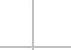
\includegraphics[max width=\textwidth]{2024_11_21_7b5527312ea89ae66fd0g-24(4)}
 &  &  & 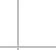
\includegraphics[max width=\textwidth]{2024_11_21_7b5527312ea89ae66fd0g-24(2)}
 &  \\
\hline
 &  &  &  &  &  &  &  &  &  &  &  &  &  &  &  &  &  &  &  &  &  &  &  &  &  &  \\
\hline
 &  &  &  &  &  &  &  &  &  &  &  &  &  &  &  &  &  &  &  &  &  &  &  &  &  &  \\
\hline
 &  &  &  &  &  &  &  &  &  &  &  &  &  &  &  &  &  &  &  &  &  &  &  &  & 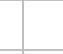
\includegraphics[max width=\textwidth]{2024_11_21_7b5527312ea89ae66fd0g-24(6)}
 &  \\
\hline
 &  &  &  &  &  &  &  &  &  &  &  &  &  &  &  &  &  &  &  &  &  &  &  &  &  &  \\
\hline
 &  &  &  &  &  &  &  &  &  &  &  &  &  &  &  &  &  &  &  &  &  &  &  &  &  &  \\
\hline
 &  &  &  &  &  &  &  &  &  &  &  &  &  &  &  &  &  &  &  &  &  &  &  &  &  &  \\
\hline
 &  &  &  &  &  &  &  &  &  &  &  &  &  &  &  &  &  &  &  &  &  &  &  &  &  &  \\
\hline
 &  &  &  &  &  &  &  &  &  &  &  &  &  &  &  &  &  &  &  &  &  &  &  &  &  &  \\
\hline
 &  &  &  &  &  &  &  &  &  &  &  &  &  &  &  &  &  &  &  &  &  &  &  &  &  &  \\
\hline
 &  &  &  &  &  &  &  &  &  &  &  &  &  &  &  &  &  &  &  &  &  &  &  &  & 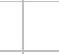
\includegraphics[max width=\textwidth]{2024_11_21_7b5527312ea89ae66fd0g-24}
 &  \\
\hline
 &  &  &  &  &  &  &  &  &  &  &  &  &  &  &  &  &  &  &  &  &  &  &  &  & 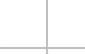
\includegraphics[max width=\textwidth]{2024_11_21_7b5527312ea89ae66fd0g-24(5)}
 &  \\
\hline
 &  &  &  &  &  &  &  &  &  &  &  &  &  &  &  &  &  &  &  &  &  &  &  &  &  &  \\
\hline
 &  &  &  &  &  &  &  &  &  &  &  &  &  &  &  &  &  &  &  &  &  & 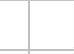
\includegraphics[max width=\textwidth]{2024_11_21_7b5527312ea89ae66fd0g-24(1)}
 &  &  & 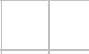
\includegraphics[max width=\textwidth]{2024_11_21_7b5527312ea89ae66fd0g-24(3)}
 &  \\
\hline
 &  &  &  &  &  &  &  &  &  &  &  &  &  &  &  &  &  &  &  &  &  &  &  &  &  &  \\
\hline
 &  &  &  &  &  &  &  &  &  &  &  &  &  &  &  &  &  &  &  &  &  &  &  &  &  &  \\
\hline
\end{tabular}
\end{center}

\begin{center}

\includegraphics[max width=\textwidth]{2024_11_21_7b5527312ea89ae66fd0g-25}
\end{center}

Odpowiedź:

\begin{center}
\begin{tabular}{|c|l|c|}
\hline
\multirow{2}{*}{\begin{tabular}{l}
Wypetnia \\
egzaminator \\
\end{tabular}} & Nr zadania & 34. \\
\cline { 2 - 3 }
 & Maks. liczba pkt & 4 \\
\cline { 2 - 3 }
 & Uzyskana liczba pkt &  \\
\hline
\end{tabular}
\end{center}

\section*{BRUDNOPIS (nie podlega ocenie)}

\end{document}